\sectionplain{Distribution}
\label{sec:distribution}

\subsection{Motivating Application}
\label{ssec:motivating-application}

\paragraph{Fraud detection}
Suppose there are two types of input events: bank transactions and fraud detection rules
that are used to flag some transactions as fraudulent. Bank
transactions are continuously input in the system with high rate while new
fraud detection rules arrive infrequently. An example of a new rule would
be the addition of a specific account to an index of suspicious accounts.
There is no way to partition inputs while
avoiding cross-partition dependencies since all events (both
transactions and rules) depend on previous rule events. Still, if the
rate of bank transaction events becomes a bottleneck (and fraud
detection rule events happen rarely) it would be beneficial to
parallelize the processing of bank transaction events.

One of the solutions that has been used to achieve data parallelism in
such computations involves extending the dataflow model with a
\emph{broadcast} pattern that allows sending some input events to \emph{all}
parallel shards (and partitioning the rest of the events as usual). An
example execution of the above computation that utilized the broadcast
pattern is shown in \Cref{fig:broadcast-dependencies-vis}. By
broadcasting the fraud detection rule events, a parallel implementation
is achieved without requiring cross-instance communication between the
parallel instances since dependencies are contained in a single
shard. However, as we see below, this solution does not generalize to
more complex dependencies.

\begin{figure}[t]
    \centering
    \begin{subfigure}[t]{0.45\textwidth}
        \centering \footnotesize{}
        \scalebox{0.8}{
        \begin{tikzpicture}[node distance=0.9cm and 0.9cm, on grid]
        %% Top Events
        \node[W] (w1) {$\textrm{Worker}_1$};
        \node[right=1.1 of w1] {$\ldots$};
        \node[B,right=1.7 of w1] (fdr1) {$\textrm{fdr}_1$};
        \node[B,right = of fdr1] (bt1) {$\textrm{bt}_1$};
        \node[B,right = of bt1] (bt2) {$\textrm{bt}_2$};
        \node[B,right=2.1 of bt2] (fdr2) {$\textrm{fdr}_2$};
        \node[B,right = of fdr2] (bt6) {$\textrm{bt}_6$};
        \node[right=0.6 of bt6] {$\ldots$};
        %% Bottom Events
        \node[W,below=1.5 of w1] (w2) {$\textrm{Worker}_2$};
        \node[right=1.1 of w2] {$\ldots$};
        \node[B,right=1.7 of w2] (fdr1') {$\textrm{fdr}_1$};
        \node[B,right = of fdr1'] (bt3) {$\textrm{bt}_3$};
        \node[B,right = of bt3] (bt4) {$\textrm{bt}_4$};
        \node[B,right = of bt4] (bt5) {$\textrm{bt}_5$};
        \node[B,right=1.2 of bt5] (fdr2') {$\textrm{fdr}_2$};
        \node[right=0.6 of fdr2'] {$\ldots$};
        %% Broadcasted events
        \node[B,above left=0.9 and 0.6 of fdr1] (fdr1root) {$\textrm{fdr}_1$};
        \node[left= of fdr1root] (broadcastfdr1) {$\textrm{broadcast}$};
        \draw[dashed,->] (fdr1root) to [out=280,in=160] (fdr1);
        \draw[dashed,->] (fdr1root) to [out=270,in=130] (fdr1');
        \node[B,above left=0.9 and 0.6 of fdr2] (fdr2root) {$\textrm{fdr}_2$};
        \node[left= of fdr2root] (broadcastfdr2) {$\textrm{broadcast}$};
        \draw[dashed,->] (fdr2root) to [out=280,in=160] (fdr2);
        \draw[dashed,->] (fdr2root) to [out=270,in=130] (fdr2');
        %% Top Edges
        \draw[E] (fdr1) -- (bt1);
        \draw[E] (fdr1) to [out=35,in=145] (bt2);
        \draw[E] (fdr1) to [out=335,in=205] (bt6);
        \draw[E] (fdr2) -- (bt6);
        %% Bottom Edges
        \draw[E] (fdr1') -- (bt3);
        \draw[E] (fdr1') to [out=35,in=145] (bt4);
        \draw[E] (fdr1') to [out=330,in=210] (bt5);
        \end{tikzpicture}
        }
        \caption{Fraud detection.}
    	\label{fig:broadcast-dependencies-vis}
	\end{subfigure}
    %
    %     \begin{subfigure}[t]{0.8\columnwidth}
% 		\centering
% 		\includegraphics[width=\columnwidth]{broadcast-dependencies.jpg}
% 		\caption{Fraud detection.}
% 		\label{fig:broadcast-dependencies-vis}
% 	\end{subfigure}
	\hfill
	\begin{subfigure}[t]{0.45\textwidth}
        \centering \footnotesize{}
        \scalebox{0.8}{
        \begin{tikzpicture}[node distance=0.9cm and 0.9cm, on grid]
        %% Top Events
        \node[W] (w1) {$\textrm{Worker}_1$};
        \node[right=1.1 of w1] {$\ldots$};
        \node[B,right=1.7 of w1] (fdr1) {$\textrm{fdr}_1$};
        \node[B,right = of fdr1] (bt1) {$\textrm{bt}_1$};
        \node[B,right = of bt1] (bt2) {$\textrm{bt}_2$};
        \node[B,right=2.1 of bt2] (fdr2) {$\textrm{fdr}_2$};
        \node[B,right = of fdr2] (bt6) {$\textrm{bt}_6$};
        \node[right=0.6 of bt6] {$\ldots$};
        %% Bottom Events
        \node[W,below=1.5 of w1] (w2) {$\textrm{Worker}_2$};
        \node[right=1.1 of w2] {$\ldots$};
        \node[B,right=1.7 of w2] (fdr1') {$\textrm{fdr}_1$};
        \node[B,right = of fdr1'] (bt3) {$\textrm{bt}_3$};
        \node[B,right = of bt3] (bt4) {$\textrm{bt}_4$};
        \node[B,right = of bt4] (bt5) {$\textrm{bt}_5$};
        \node[B,right=1.2 of bt5] (fdr2') {$\textrm{fdr}_2$};
        \node[right=0.6 of fdr2'] {$\ldots$};
        %% Broadcasted events
        \node[B,above left=0.9 and 0.6 of fdr1] (fdr1root) {$\textrm{fdr}_1$};
        \node[left= of fdr1root] (broadcastfdr1) {$\textrm{broadcast}$};
        \draw[dashed,->] (fdr1root) to [out=280,in=160] (fdr1);
        \draw[dashed,->] (fdr1root) to [out=270,in=130] (fdr1');
        \node[B,above left=0.9 and 0.6 of fdr2] (fdr2root) {$\textrm{fdr}_2$};
        \node[left= of fdr2root] (broadcastfdr2) {$\textrm{broadcast}$};
        \draw[dashed,->] (fdr2root) to [out=280,in=160] (fdr2);
        \draw[dashed,->] (fdr2root) to [out=270,in=130] (fdr2');
        %% Top Edges
        \draw[E] (fdr1) -- (bt1);
        \draw[E] (fdr1) to [out=30,in=145] (bt2);
        \draw[E] (fdr1) to [out=30,in=160] (bt6);
        \draw[E] (bt2) -- (fdr2);
        \draw[E] (bt1) to [out=335,in=205] (fdr2);
        \draw[E] (fdr2) -- (bt6);
        %% Bottom Edges
        \draw[E] (fdr1') -- (bt3);
        \draw[E] (fdr1') to [out=35,in=145] (bt4);
        \draw[E] (fdr1') to [out=330,in=210] (bt5);
        \draw[E] (bt3) to [out=330,in=210] (fdr2');
        \draw[E] (bt4) to [out=330,in=210] (fdr2');
        \draw[E] (bt5) -- (fdr2');
        %% Cross-Dependency Edges
        \draw[red,->] (bt1) -- (fdr2');
        \draw[red,->] (bt2) -- (fdr2');
        \draw[red,->] (bt3) -- (fdr2);
        \draw[red,->] (bt4) -- (fdr2);
        \draw[red,->] (bt5) -- (fdr2);
        \end{tikzpicture}
        }
        % \centering
        % \includegraphics[width=\columnwidth]{cross-instance-dependencies.jpg}
        \caption{ML extension of fraud detection.}
        \label{fig:cross-instance-dependencies-vis}
	\end{subfigure}

% 	\begin{subfigure}[t]{0.8\columnwidth}
%         \centering
%         \includegraphics[width=\columnwidth]{cross-instance-dependencies.jpg}
%         \caption{ML extension of fraud detection.}
%         \label{fig:cross-instance-dependencies-vis}
% 	\end{subfigure}
    \caption{Illustration of an execution of two fraud detection
      examples and the event dependencies. Time progresses from left to right,
            different rows represent different parallel workers,
                  circles represent processing of
      events, dashed edges represent broadcasting an event,
            black edges represent dependencies, and red edges
      represent dependencies across parallel instances.
    %   \kk{Add an explanation of space-time in this diagram. That time moves from left to right etc.}
      }
    \label{fig:dependencies-vis}
\end{figure}



\paragraph{Fraud detection with a machine learning (ML) extension}
Consider a simple extension of the above application that is inspired
by today's ML workflows. In addition to user-input fraud detection
rules, the extended application also trains a model in an unsupervised
way using previously seen transactions. To achieve that the application keeps a sketch of previously seen bank transaction events. When a new fraud detection rule arrives, it aggregates the sketches and uses them to retrain the global fraud detection model.
As shown in
\Cref{fig:cross-instance-dependencies-vis},
this introduces dependencies across shards as the model retraining on rule events depends on all the previous bank transactions (even after broadcasting the rules), requiring communication between shards.

Unfortunately, standard ways of achieving data parallelism do not
support computations with such cyclic dependencies, leaving the user with two
unsatisfying solutions. They can either accept this
shortcoming and execute their computations with restricted parallelism---introducing
a throughput bottleneck in their application, or they can manually
implement the required synchronization using low level external
synchronization mechanisms (e.g. a key-value store with strong
consistency guarantees). This is error prone and, more importantly,
violates the implicit assumptions about the usage of
streaming APIs possibly leading to bugs and
erroneous behaviors.

\subsection{System Architecture}
\label{ssec:solution-architecture}

Our solution can achieve data parallelism for the extended fraud
detection application through the architecture
summarized in \Cref{fig:system-architecture-overview}.
The two primary abstractions (shown in blue) encode the required complex synchronization requirements at different levels of abstractions:
the DGS specification describes the computation and input dependencies
in a platform-independent manner,
and synchronization plans express the synchronization
between processes at the implementation level,
as communications between a hierarchically structured tree of processes.

The DGS specification is split in three parts.
First, the user
needs to provide a sequential implementation of the program, where the
input is assumed to arrive in order and one event at a time. The
sequential implementation consists of a stateful update function that
can output events and update its state every time an input event is
processed. For the fraud detection example, the update function would
process bank transactions by checking if they are fraudulent and by
constructing a sketch of the previously seen transactions, and fraud
detection rules by using the sketch of previously seen transactions
and the new rule to update the statistical fraud model. Second, the
user provides a dependence relation that indicates the input events
for which the processing order must be preserved, inducing a partial
order on input events. For the current example, the user would simply
indicate that fraud detection rule events depend on all other
events. The final part of a specification consists of primitives that
describe how to \emph{fork} the state into two independent copies to
allow for parallel processing and how to \emph{join} two states when
synchronization is required. These primitives abstractly represent
splitting the computation into independent computations and merging
the results, and are not tied to a specific implementation.

Given a DGS specification,
the mapping to the synchronization plan in our architecture
is given by a pluggable optimization component, which picks
a synchronization plan based on information about the target execution
environment, e.g. the number of processing workers and the location of
the input streams. All of the induced plans are shown to be correct with respect to the sequential specification, so the optimizer is free to pick any of them without endangering correctness. As a starting point, we have developed a simple
optimizer that tries to minimize the number of messages exchanged
between different workers using information about the execution
environment and the input streams.
As a final step, the synchronization plan abstraction
is deployed by the runtime system,
which among other implementation details enforces the ordering of input events based on input dependencies,
and is implemented in our DGSStream prototype.

\begin{figure}
  \centering
  \scalebox{.8}{
    \begin{tikzpicture}[scale=0.9, transform shape, auto, node distance=1cm]
      \node[Block] (user) {Programmer};
      \node[Block,Data,Input,right=of user] (spec) {DGS Specification  \\ (\S\ref{sec:prog-model})};
      \node[Block,right=of spec] (opt) {Optimizer \\ (\S\ref{ssec:optimization-problem})};
    %   \node[Block,Data,Input,right=of opt] (top) {Target \\ Topology (\S\ref{sec:dist-impl})};
      \node[Block,Data,right=of opt] (cfg) {Synchronization \\ Plan (\S\ref{ssec:distributed-configurations})};
      \node[Block,right=of cfg] (impl) {Implementation \\ (\S\ref{ssec:runtime})};
      % \node[Block,right=3cm of cfg] (cd) {Code Distributor \\ (\S\ref{ssec:runtime})};
      % \node[Block,Output,below=1.5cm of cd] (impl) {Implementation};

      \draw[Block Edge] (user) -- (spec);
      \draw[Block Edge] (spec) -- (opt);
    %   \draw[Block Edge] (top) -- (opt);
    %   \draw[Block Edge] (top) -- (impl);
      \draw[Block Edge] (opt) -- (cfg);
      \draw[Block Edge] (cfg) -- (impl);
    \end{tikzpicture}
  }
  \caption{Architecture of the end-to-end DGS framework.
  }
\label{fig:system-architecture-overview}
\end{figure}

\subsection{Dependency-Guided Synchronization (DGS)}
\label{sec:prog-model}

A DGS specification consists of three components: a
\emph{sequential specification}, a \emph{dependence relation} on input
events to enforce synchronization, and \emph{fork} and \emph{join}
parallelization primitives.
At the end of the section we define specification \emph{consistency}, which are requirements on the \emph{fork} and \emph{join} functions to ensure that any parallelized implementation generated from the specification is equivalent to the sequential one.
As specifications are given programmatically,
we also refer to DGS as a \emph{programming model} and
to specifications as \emph{programs}.

\subsubsection{Walkthrough}

For a simple but illustrative example, suppose that we want to
implement a stream processing application that simulates a map from
keys to counters, in which there are two types of input events: \emph{increment}
events, denoted $\tg{i}(k)$, and \emph{read-reset} events, denoted
$\tg{r}(k)$, where each event has an associated key $k$.  On each
increment event, the counter associated with that key should be
increased by one, and on each read-reset event, the current value of
the counter should be produced as output, and then the counter should be reset to
zero.
The ``type'' of an input event is called its \emph{tag}, and in this example there are
two tags.
An input event may also carry a \emph{payload} of data that is not
used for parallelization. In this example all events have an empty payload.

\paragraph{Sequential specification.}
\label{p:seq-impl}
In our programming model, the user first provides a sequential
implementation of the desired computation.
A pseudocode version of the sequential specification for the
example above is shown in \Cref{fig:key-value-store} (left). It consists of
(i) the state type \fl{State}, i.e. the map from keys to
counters, (ii) the initial value of the state \fl{init},
i.e. $0$ for all keys, and (iii) a function \fl{update},
which contains the logic for processing input events.
Conceptually, the sequential specification describes how to process
the data assuming it was all combined into a single sequential stream (e.g.,
sorted by system timestamp).  For example, if the input stream
consists of the events $\tg{i}(1), \tg{i}(2), \tg{r}(1), \tg{i}(2),
\tg{r}(1)$, then the output would be $1$ followed by $0$, produced by
the two $\tg{r}(1)$ (read-reset) events.

\begin{figure}[t]
\centering \footnotesize{}
\begin{minipage}{0.38\textwidth}
\begin{FluminaCode}
// Types
Key = Integer
Tag = i(Key) | r(Key)
Payload = ()
Event = (Tag, Payload)
State = Map(Key, Integer)




// Sequential Implementation
init: () -> State
init() =
    return emptyMap()
update: (State, Event) -> State
update(s, (i(k), ())) =
    s[k] = s[k] + 1;
    return s
update(s, (r(k), ())) =
    output s[k];
    s[k] = 0;
    return s
\end{FluminaCode}
\end{minipage}
\begin{minipage}{0.6\textwidth}
\begin{FluminaCode}
// Dependence Relation
dependencies: (Tag, Tag) -> Bool
dependencies(r(k1), r(k2)) = k1 == k2
dependencies(r(k1), i(k2)) = k1 == k2
dependencies(i(k1), r(k2)) = k1 == k2
dependencies(i(k1), i(k2)) = false

// Fork and Join
fork: (State, Tag -> Bool, Tag -> Bool) -> (State, State)
fork(s, pred1, pred2) =
    s1 = init(); s2 = init() // two forked states
    for k in keys(s):
        if pred1(r(k)):
            s1[k] = s[k]
        else: // pred2(r(k)) OR r(k) in neither
            s2[k] = s[k]
    return (s1, s2)
join: (State, State) -> State
join(s1, s2) =
    for k in keys(s2):
        s1[k] = s1[k] + s2[k]
    return s1
\end{FluminaCode}
\end{minipage}


\caption{
  Specification in DGS of a map from keys to counters, which
  can process increment operations $\tg{i}(k)$ and read-reset
  operations $\tg{r}(k)$ for each key $k$.
  Erlang syntax has been
  edited for readability.
  We use \fl{s[k]} as shorthand for getting key $k$ from the map
  \emph{or} the default value $0$ if it is not present.
}
\label{fig:key-value-store}
\end{figure}

\begin{figure}
    \centering
    \scriptsize{}
    \begin{tabular}{cc}
        \TwoTagDepGraph{\tg{r}(1)}{\tg{i}(1)}{\draw (1) edge[Tag Loop] (1); \draw (1) edge[Tag Edge] (2);}
      & \TwoTagDepGraph{\tg{r}(2)}{\tg{i}(2)}{\draw (1) edge[Tag Loop] (1); \draw (1) edge[Tag Edge] (2);} \\
        % \TwoTagDepGraph{\tg{r}(3)}{\tg{i}(3)}{\draw (1) edge[Tag Loop] (1); \draw (1) edge[Tag Edge] (2);} \\
        \multicolumn{2}{c}{$\cdots$}
    \end{tabular}
    \captionof{figure}{The \fl{dependencies} relation from \Cref{fig:key-value-store}
    visualized as a graph, with 2 keys shown.
    Edges enforce synchronization requirements, while non-edges expose parallelism.}
    \label{fig:key-value-store-dependencies}
\end{figure}

\paragraph{Dependence relation.}
%
To parallelize a sequential computation, the user needs to provide a
dependence relation which encodes which events are independent, and
thus can be processed in parallel, and which events are dependent, and
therefore require synchronization.  The dependence relation abstractly
captures all the dependency patterns that appear in an application,
inducing a partial order on input events. In this example, there are
two forms of independence we want to expose. To begin with,
\emph{parallelization by key} is possible: the counter map could be
partitioned so that events corresponding to different sets of keys are processed
independently. Moreover, \emph{parallelizing increments} on the
counter of the same key is also possible. In particular, different
sets of increments for the same key can be processed independently; we
only need to aggregate the independent counts when a read-reset
operation arrives. On the other hand, read-reset events
are synchronizing for a particular key;
their output is affected by the processing of increments
as well as other read-reset events of that key.

% \begin{figure}
% \centering \scriptsize{}
% \begin{tabular}{cccc}
%   \TwoTagDepGraph{\tg{r}(1)}{\tg{i}(1)}{\draw (1) edge[Tag Loop] (1); \draw (1) edge[Tag Edge] (2);}
% & \TwoTagDepGraph{\tg{r}(2)}{\tg{i}(2)}{\draw (1) edge[Tag Loop] (1); \draw (1) edge[Tag Edge] (2);}
% & \TwoTagDepGraph{\tg{r}(3)}{\tg{i}(3)}{\draw (1) edge[Tag Loop] (1); \draw (1) edge[Tag Edge] (2);}
% & $\cdots$
% \end{tabular}
% \caption{The \fl{dependencies} relation from \Cref{fig:key-value-store}
% visualized as a graph, with 3 keys shown.
% Edges enforce synchronization requirements, while non-edges expose parallelism.}
% \label{fig:key-value-store-dependencies}
% \end{figure}

We capture this combination of parallelization and synchronization
requirements by defining the dependence relation
\fl{dependencies} in \Cref{fig:key-value-store}, which is
also visualized in \Cref{fig:key-value-store-dependencies}.
In the specification, the set of tags may be \emph{symbolic}
(infinite): here \fl{Tag} is parameterized by an integer \fl{Key}.
To allow for this, the dependence relation
is formally a \emph{predicate} on pairs of tags,
and is given programmatically as a function from pairs
of \fl{Tag} to \fl{Bool}.
For example, \fl{dependencies(r(k1), r(k2))} (one of four cases)
is given symbolically as equality comparison of keys, \fl{k1 == k2}.
The dependence relation should also be \emph{symmetric},
i.e. \fl{e1} is in \fl{dependencies(e2)} if and
only if \fl{e2} is in \fl{dependencies(e1)}.

\paragraph{Parallelization primitives: \emph{fork} and \emph{join}.}
\label{p:fork-join}
%
While the dependence relation indicates the possibility of
parallelization, it does not provide a mechanism for parallelizing
state.  The parallelization is specified using a pair of functions to \fl{fork}
one state into two, and to \fl{join} two states into one.
The
fork function additionally takes as input two predicates of tags,
such that the two predicates are \emph{independent} (but not necessarily disjoint):
every tag satisfying \fl{pred1} is independent of every tag satisfying \fl{pred2}.
The
contract is that after the state is forked into two independent
states, each state will then \emph{only be updated using events from
the given set of tags.}
A fork-join specification for our example
is shown in~\cref{fig:key-value-store}.
The \fl{join} function simply adds up the counts for each key to form the combined
state. The \fl{fork} function has to decide, for each key, which forked state
to send the count to.
Since read-reset operations \fl{r(k)} are synchronizing and require knowing the total count,
it does this by checking
which forked state is responsible for processing read-reset
operations, if any.

It is necessary that the \fl{fork} function
have the predicates \fl{pred1} and \fl{pred2} as input,
as otherwise we would not know how to partition the state \fl{s}
in case of \emph{parallelization by key}.
For example, if \fl{pred1} contains all events of key $1$
and \fl{pred2} contains all events of key $2$,
then we need to propagate the count \fl{s[1]} to the first forked state
and the count \fl{s[2]} to the second forked state.
However, it is also possible that \fl{pred1} and \fl{pred2}
are \emph{not} disjoint,
which is necessary to accommodate \emph{parallelization by increment}.
For example, \fl{pred1} and \fl{pred2} may both contain \fl{i(3)}
events.
This is the reason that we include both \fl{pred1} and \fl{pred2},
even though only \fl{pred1} is used in our example.
Fortunately in this case, the independence requirement
guarantees that neither forked state will be responsible for
\fl{r(3)} events (as \fl{r(3)} is dependent on \fl{i(3)});
in particular, neither forked state will be required to produce output for key $3$.
Therefore, we can choose to propagate the count \fl{s[3]} to either state,
knowing that the two forked counts will later be added back together in \fl{join}.
% as long as we ensure the counts are added when the states are joined back together.
This illustrates that the fork function's input can indicate either
a partitioning of input events, or parallelization on events on the same tag
(or a combination of these across different keys).
% This information is encoded using a pair of predicates
% (and cannot be encoded using only one).


% For our specific example, the guarantee is that only one of two
% forked states will be assigned to process read-reset events for a key. If the
% input $\tg{r}(k)$ is in \fl{tags1}, then we know that
% updates of key $k$ will all be processed by the first state, and so we
% copy the value for this key to the first state. Conversely, if the
% input $\tg{r}(k)$ is in \fl{tags2}, we copy the value for
% this key to the second state.  The third case is that the input
% $\tg{r}(k)$ is in neither \fl{tags1} nor
% \fl{tags2}; then we can copy the value to \emph{either} the
% first or the second state. In this case, both states may receive
% increment events. This is acceptable because before any read-reset
% operation can be processed, the \fl{join} function will be
% called, which adds the two totals back together again.

\begin{figure}
\centering \scriptsize{}
% \scalebox{0.8}{
\begin{tikzpicture}[node distance=0.9cm and 0.9cm, on grid]
%% Bottom Nodes
\node[B] (0) {$\istate$};
\node[B,right = of 0] (1) {${\tg{r}(1)}$};
\node[B,right = of 1] (2) {$\fk$};
\node[B,below right = of 2] (2b) {${\tg{i}(1)}$};
\node[B,right = of 2b] (3) {$\fk$};
\node[B,above = of 3] (2a) {${\tg{i}(1)}$};
\node[B,below right = of 3] (3b) {${\tg{i}(1)}$};
\node[B,above right = of 3b] (4) {$\jn$};
\node[B,above right = of 4] (5) {$\jn$};
\node[B,right = of 5] (6) {${\tg{r}(1)}$};
\coordinate[right=0.5cm of 6] (7);
%% Top Nodes
\node[B,above = of 0] (t0) {$\istate$};
\node[B,right = of t0] (t1) {${\tg{r}(1)}$};
\node[B,above right = of 2] (t2) {${\tg{i}(1)}$};
\node[B,right = of t2] (t3) {${\tg{i}(1)}$};
\node[B,right = of t3] (t4) {${\tg{i}(1)}$};
\node[B,above = of 6] (t5) {${\tg{r}(1)}$};
\coordinate[right=0.5cm of t5] (t6);
%% Bottom Edges
\draw[E] (0) -- (1);
\draw[E] (1) -- (2);
\draw[E] (2) -- (2a);
\draw[E] (2) |- (2b);
\draw[E] (2b) -- (3);
\draw[E] (3) -- (4);
\draw[E] (3) |- (3b);
\draw[E] (3b) -| (4);
\draw[E] (4) -| (5);
\draw[E] (2a) -- (5);
\draw[E] (5) -- (6);
\draw[E] (6) -- (7);
%% Top Edges
\draw[E] (t0) -- (t1);
\draw[E] (t1) -- (t2);
\draw[E] (t2) -- (t3);
\draw[E] (t3) -- (t4);
\draw[E] (t4) -- (t5);
\draw[E] (t5) -- (t6);
\end{tikzpicture}
% }
\caption{Example of a sequential and parallel execution of the program in \cref{fig:key-value-store} on the input stream $\tg{r}(1), \tg{i}(1), \tg{i}(1), \tg{i}(1), \tg{r}(1)$. Here $k = 1$ is a key, and
$\fk$ and $\jn$ denote fork and join functions.
\emph{\textbf{Top:} Sequential execution: each item of the input stream is processed as an update to a global state. \textbf{Bottom:} One possible parallel execution: in between some updates, the state is forked or joined, and $\tg{i}$ events are processed as independent updates to one of the forked states.}}
\label{fig:example-wire-diagram}
\end{figure}

\subsubsection{Formal Definition}

A DGS specification can be more general than we have discussed so far,
because we allow for multiple \emph{state types}, instead of just
one. The initial state must be of a certain type, but forks and joins
can convert from one state type to another: for example, forking a
pair into its two components.
Additionally,
each state type can come with a \emph{predicate} which restricts
the allowed tags processed by a state of that type.
The complete programming model is summarized in the following
definition.

\begin{definition}[DGS Specification]
\label{def:prog-model}
Let \fl{Pred(T)} be a given type of \emph{predicates}
on a type \fl{T},
where predicates denote functions \fl{T -> Bool}.
A specification consists of the following components:
\begin{enumerate}[(1)]
\item A type of input events \fl{Event = (Tag, Payload)},
where \fl{Tag} is a type of tags.
\item The dependence relation \fl{dependencies: Pred(Tag, Tag)},
which is symmetric: \fl{dependencies(tag1, tag2)}
iff \fl{dependencies(tag2, tag1)}.
\item A type for output events \fl{Out}.
\item Finitely many state types \fl{State_0}, \fl{State_1}, etc.
\item For each state type \fl{State_i},
a predicate \fl{pred_i: Pred(Tag)} --- this specifies which input values this type of state can process --- where \fl{pred_0} $=$ \fl{true}.
\item A sequential implementation, consisting of a single initial state \fl{init: State_0} and for each state type \fl{State_i},
a function \fl{update_i: (State_i, Event) -> State_i}.
The update also produces zero or more outputs, given formally by a function
\fl{out_i: (State_i, Event) -> List(Out)}.
\item Any number of parallelization primitives, where each is either a \emph{fork} or a \emph{join}. A fork function has type
\fl{(State_i, Pred(Tag), Pred(Tag)) -> (State_j, State_k)},
and a join function has type
\fl{(State_j, State_k) -> State_i}, for some $i, j, k$.
\end{enumerate}
\end{definition}

The semantics of a specification
can be visualized using wire
diagrams, as in \Cref{fig:example-wire-diagram}. Computation proceeds from left to right. Each wire is associated with
(i) a state (of type \fl{State_i} for some $i$) and
(ii) a predicate on tags (of type \fl{Pred(Tag)})
which restricts the input events that this wire can process.
Input events are processed as
updates to the state, which means they take one input wire and produce
one output wire, while forks take one input wire and produce two, and
joins take two input wires and produce one. Notice that the same updates are present in both sequential and parallel executions. It is guaranteed in the
parallel execution that \emph{fork and join come in pairs}, like
matched parentheses. Each predicate on tags that is given as input to the \fl{fork} function indicates the set of input events that can be processed along one of the outgoing wires.
Additionally, we require that updates on parallel wires must be
on independent tags.
In the example,
the wire is forked into two parts and then forked again, and all three
resulting wires process $\tg{i}(1)$ events. Note that $\tg{r}(1)$
events cannot be processed at that time because they are dependent on
$\tg{i}(1)$ events.
More specifically, we require that
the predicate at each wire of type \fl{State_i}
implies \fl{pred_i}, and that
after each \fl{fork} call,
the predicates at each resulting wire denote independent sets of tags.
This semantics is formalized in the following definition.

\begin{definition}[DGS Semantics]
\label{def:prog-model-semantics}
A \emph{wire} is a triple
\wire{\fl{State_i}}{\fl{pred}}{\fl{s}},
where
\fl{State_i} is a state type,
\fl{s: State_i},
and \fl{pred: Pred(Tag)}
is a predicate of allowed tags,
such that \fl{pred} implies \fl{pred_i}.
We give the semantics of a specification through an
inductively defined relation, which we denote
\semantics{\fl{State}}{\fl{pred}}{\fl{s}}{\fl{u}}{\fl{s'}}{\fl{v}},
where
\wire{\fl{State}}{\fl{pred}}{\fl{s}} and \wire{\fl{State}}{\fl{pred}}{\fl{s'}}
are the starting and ending wires
(with the same state type and predicate),
\fl{u: List(Event)} is an input stream,
and \fl{v: List(Out)} is an output stream.
Let \fl{l1 + l2} be list concatenation, and
define \fl{inter(l, l1, l2)} if \fl{l} is some interleaving of \fl{l1} and \fl{l2}.
For \fl{e1}, \fl{e2: Event},
let \fl{indep(e1, e2)} denote that
\fl{e1} and \fl{e2} are not dependent, i.e.
\fl{not(dependencies(}\fst{\fl{e1}}\fl{,}\fst{\fl{e2}}\fl{))}.
There are two base cases and two inductive cases.
\begin{itemize}
\item (Emp)
For any \fl{State}, \fl{pred}, and \fl{s},
\semantics{\fl{State}}{\fl{pred}}{\fl{s}}{\fl{[]}}{\fl{s}}{\fl{[]}}.
\item (Upd)
For any \fl{State}, \fl{pred}, \fl{s}, and any \fl{e: Event},
if the tag of \fl{e} satisfies \fl{pred}, i.e.
\fl{pred(}\fst{\fl{e}}\fl{)}, then
\semantics{\fl{State}}{\fl{pred}}{\fl{s}}{\fl{[e]}}{\fl{update(s, e)}}{\fl{out(s, e)}}.
\item (Seq)
For any \fl{State}, \fl{pred}, \fl{s}, \fl{s'}, \fl{s''},
\fl{u}, \fl{v}, \fl{u'}, and \fl{v'}, if
\semantics{\fl{State}}{\fl{pred}}{\fl{s}}{\fl{u}}{\fl{s'}}{\fl{v}}
and
\semantics{\fl{State}}{\fl{pred}}{\fl{s'}}{\fl{u'}}{\fl{s''}}{\fl{v'}},
then
\semantics{\fl{State}}{\fl{pred}}{\fl{s}}{\fl{u + u'}}{\fl{s''}}{\fl{v + v'}}.
\item (Par)
Lastly, for any
\fl{State}, \fl{State1}, \fl{State2},
\fl{pred}, \fl{pred1}, \fl{pred2},
\fl{s},
\fl{s1'}, \fl{s2'},
\fl{u}, \fl{u1}, \fl{u2}, \fl{v}, \fl{v1}, \fl{v2},
\fl{fork}, and \fl{join},
suppose that
(the conjunction) \fl{pred1(e1)} and \fl{pred2(e2)} implies
\fl{indep(e1, e2)},
\fl{pred1} implies \fl{pred}, and
\fl{pred2} implies \fl{pred}.
Let
\fl{fork(s, pred1, pred2) = (s1, s2)}
and
\fl{join(s1', s2') = s'},
and suppose that
\fl{inter(u, u1, u2)}
and
\fl{inter(v, v1, v2)}.
If
\semantics{\fl{State1}}{\fl{pred1}}{\fl{s1}}{\fl{u1}}{\fl{s1'}}{\fl{v1}}
and
\semantics{\fl{State2}}{\fl{pred2}}{\fl{s2}}{\fl{u2}}{\fl{s2'}}{\fl{v2}}
then
\semantics{\fl{State}}{\fl{pred}}{\fl{s}}{\fl{u}}{\fl{s'}}{\fl{v}}.
\end{itemize}
The \emph{semantics} $\sem{S}$ of the specification $S$
is the set of pairs $(\fl{u}, \fl{v})$
of an input stream \fl{u} and an output stream \fl{v} such that
\semantics{\fl{State_0}}{\fl{true}}{\fl{init}}{\fl{u}}{\fl{s'}}{\fl{v}}
for some final state \fl{s'}.
\end{definition}

\subsubsection{Consistency of Specifications}
\label{ssec:prog-model-correctness}

Any parallel execution
is guaranteed to preserve the sequential semantics, i.e. processing
all input events \emph{in order} using the \fl{update} function,
as long as the following \emph{consistency conditions} are
satisfied.
The sufficiency of these conditions is shown in
\Cref{thm:consistency-implies-determinism}, which states
that \emph{consistency implies determinism up to output reordering}.
This is a key step in the end-to-end proof of correctness in \Cref{ssec:proof-of-correctness}.
Consistency can be thought of as analogous to the commutativity and
associativity requirements for a MapReduce program to have
deterministic output~\cite{dean2008mapreduce}: just as with MapReduce
programs, the implementation does \emph{not} assume the conditions are
satisfied, but if not the semantics will be dependent on how the
computation is parallelized.

Let us briefly illustrate the consistency conditions for our running example
(\Cref{fig:key-value-store}).
% consider (C1), which states that joins commute with updates.
If \fl{e} is an increment event,
then condition (C1) captures the fact that counting can be done in parallel:
it reduces to $\fl{(s1[k] + s2[k]) + 1} = \fl{(s1[k] + 1) + s2[k]}$.
% For a read-reset event, this holds due to an invariant on the state
% s2[k] that it must be 0 for that key because the key for s1[0] is 0.
Condition (C2) captures the fact that we preserve total count
across states when forking: it reduces to $\fl{s[k] + 0} = \fl{s[k]}$.
Condition (C3) would not be valid for \emph{general} events
\fl{e1}, \fl{e2}, because a read-reset event does not commute with an increment
of the same key ($\fl{s[k] + 1} \ne \fl{s[k]}$),
hence the restriction that \fl{indep(e1, e2)}.
Finally, one might think that a variant of (C1) should hold for
\fl{fork} in addition to \fl{join},
but this turns out not to be the case:
for example, starting from $\fl{s[k] = 100}$,
an increment followed by a fork might yield the pair of counts
$(101, 0)$, while a fork followed by an increment might yield
$(100, 1)$.
It turns out however that commutativity only with joins, and not with
forks, is enough to imply \Cref{thm:consistency-implies-determinism}.

\begin{definition}[Consistency]
\label{def:prog-model-consistency}
A specification is \emph{consistent} if the following
equations always hold:
\begin{align*}
\fl{join(update(s1, e), s2)}
    &\;= \fl{update(join(s1, s2), e)} \tag{C1} \\
\fl{join(fork(s, pred1, pred2))}
    &\;= \fl{s} \tag{C2} \\
\fl{update(update(s, e1), e2))}
    &\;= \fl{update(update(s, e2), e1))}. \tag{C3}
\end{align*}
Equation (C1)
is over all
join functions \fl{join: (State_j, State_k) -> State_i},
events \fl{e: Event} such that \fl{pred_i(e)} and \fl{pred_j(e)},
and states \fl{s1: State_j}, \fl{s2: State_k},
where \fl{update} denotes the update function on the appropriate type.
Additionally the corresponding output on both sides must be the same:
$\fl{out(s1, e)} = \fl{out(join(s1, s2))}$.
Equation (C2)
is over all
fork functions \fl{fork: (State_i, Pred(Tag),} \fl{Pred(Tag)) -> (State_j, State_k)}
join functions \fl{join: (State_j, State_k) -> State_i},
states \fl{s: State_i}, and predicates \fl{pred1} and \fl{pred2}.
Equation (C3)
is over all state types \fl{State_i},
states \fl{s: State_i},
and \emph{independent} events
\fl{indep(e1, e2)}
such that \fl{pred_i(e1)} and \fl{pred_i(e2)}.
As with (C1), we also require that the outputs
agree:
$\fl{out(s, e1) + out(update(s, e1), e2) = out(update(s, e2), e1) + out(s, e2)}$.
\end{definition}


%% Form of definition using enumerate
% \begin{definition}[Consistency]
% \label{def:prog-model-consistency}
% A specification is \emph{consistent} if the following
% three conditions hold.
% \begin{enumerate}[(1)]
% \item
% For all
% join functions \fl{join: (State_j, State_k) -> State_i},
% events \fl{e: Event} such that \fl{pred_i(e)} and \fl{pred_j(e)},
% states \fl{s1: State_j} and \fl{s2: State_k},
% where \fl{update} denotes the update function on the appropriate type:
% \[
% \fl{join(update(s1, e), s2)} = \fl{update(join(s1, s2), e)}, \tag{1}
% \]
% and the corresponding output on both sides is the same:
% $\fl{out(s1, e)} = \fl{out(join(s1, s2))}$.
% \item
% For all
% fork functions \fl{fork: (State_i, Pred(Tag), Pred(Tag)) -> (State_j, State_k)}
% join functions \fl{join: (State_j, State_k) -> State_i},
% states \fl{s: State_i}, and predicates \fl{pred1} and \fl{pred2},
% \[
% \fl{join(fork(s, pred1, pred2))} = \fl{s}. \tag{2}
% \]
% \item
% For all state types \fl{State_i},
% states \fl{s: State_i},
% and events \fl{e1}, \fl{e2: Event}
% such that \fl{pred_i(e1)} and \fl{pred_i(e2)},
% \emph{if} \fl{indep(e1, e2)} then
% \[
% \fl{update(update(s, e1), e2))} = \fl{update(update(s, e2), e1))}, \tag{3}
% \]
% and the corresponding output on both sides
% is the same:
% $\fl{out(s, e1)} + \fl{out(update(s, e1), e2)}
% = \fl{out(update(s, e2), e1)} + \fl{out(s, e2)}$.
% \end{enumerate}
% \end{definition}

%% Definition using single align* equation for all 5 conditions
% for all functions \fl{update}, \fl{out}, \fl{join}, and \fl{fork}
% in the specification:
% \begin{align*}
% \fl{join(update(s1, e), s2)}
%     =\;& \fl{update(join(s1, s2), e)}
%     \tag{1a} \\
% \fl{out(s1, e)}
%     =\;& \fl{out(join(s1, s2))}
%     \tag{1b} \\
% \fl{join(fork(s, pred1, pred2))}
%     =\;& \fl{s} \tag{2} \\
% \fl{update(update(s, e1), e2))}
%     =\;& \fl{update(update(s, e2), e1))}
%     \tag{3a} \\
% \fl{out(s, e1)} + \fl{out(update(s, e1), e2)}
%     =\;& \fl{out(update(s, e2), e1)} + \fl{out(s, e2)}
%     \tag{3b}
% \end{align*}

\begin{theorem}
\label{thm:consistency-implies-determinism}
If $S$ is consistent, then $S$ is deterministic up to output reordering:
that is,
for all $(\fl{u}, \fl{v}) \in \sem{S}$,
\fl{set(v) = set(spec(u))}.
\end{theorem}
\begin{proof}
We show by induction on the semantics in \Cref{def:prog-model-semantics}
that every wire diagram is equivalent (up to output reordering) to the sequential sequence
of updates.
The (Seq) inductive step is direct by associativity of function composition
on the left and right sequence of updates (no commutativity of updates is required).
For the (Par) inductive step, we replace the two parallel wires with sequential wires,
then apply (C1) repeatedly on the last output to move it outside of the parallel wires,
then finally apply (C2) to reduce the now trivial parallel wires to a single wire.
% Caleb: I think that consistency condition C3 is actually unused, interestingly enough.
% I won't mention it in the proof sketch since I might have missed something.
\end{proof}

\subsection{Distributed Implementation}
\label{sec:dist-impl}

This section describes the distributed runtime for DGS.
In particular, we describe \emph{synchronization plans},
which represent streaming program implementations, and our
framework for generating them from the given DGS specification
in \cref{sec:prog-model}.
Generation of an implementation can be
conceptually split in two parts, the first ensuring correctness and
the second affecting performance. First a specification $S$ induces a set of
$S$-\emph{valid}, i.e. correct with respect to it, synchronization
plans. Choosing one of those plans is then an independent optimization
problem that does not affect correctness and can be delegated to a
separate optimization component (\cref{ssec:optimization-problem}).
Finally, the workers in synchronization plans
need to process some incoming events in order while some can be
processed out of order (depending on the dependence relation).  We
propose a selective reordering technique
(\cref{ssec:runtime}) that can be used in tandem with heartbeats to
address this ordering issue.
We tie everything together by providing an end-to-end proof that the
implementation is correct with respect to a consistent specification
$S$ (and importantly, independent of the synchronization plan chosen
as long as it is $S$-valid) in \cref{ssec:proof-of-correctness}.
Before describing the separate framework components, we first
articulate the necessary underlying assumptions about input streams in
\cref{ssec:distributed-assumptions}.

\subsubsection{Preliminaries}
% \subsubsection{Streaming Assumptions}
\label{ssec:distributed-assumptions}

In our model the input is partitioned in some number of input streams that could be distributed, i.e. produced at different locations.
We assume that the implementation has access to \emph{some} ordering
relation $\mathcal{O}$ on pairs of input events (also denoted
$<_{\mathcal{O}}$), and the order of events is increasing along each
input stream. This is necessary for cases where the
\emph{user-written} specification requires that events arriving in
different streams are dependent, since it allows the implementation to
have progress and process these dependent events in order.
Concretely, in our setting $\mathcal{O}$ is implemented using \emph{event timestamps}.
Note that these timestamps do not need to correspond to real time, if this is not required by the application.
In cases where real-time timestamps are required, this can be achieved with well-synchronized clocks, as has been done in other systems, e.g. Google Spanner~\cite{corbett2013spanner}.

%% % To clarify why this is not overly restrictive, suppose for example that the implementation has two streams arriving at different nodes, and some events $x_1$ and $x_2$ arrive on stream 1 and stream 2, respectively. There are two cases. First if $x_1$ and $x_2$ are independent (and the user has written a fork function), then the system could fork state to process them in parallel, so the order relation is ignored and not necessary. Second, if they are dependent, then this means that we need to synchronize and process $x_1$ and $x_2$ sequentially.
%% % In this synchronizing case, we process $x_1$ first if $x_1 <_{\mathcal{O}} x_2$ and $x_2$ first if $x_2 <_{\mathcal{O}} x_1$, irrespective of the time that $x_1$ and $x_2$ arrive in the system, which makes the execution deterministic.
%% % The increasing condition (2) is necessary to ensure progress: in the synchronizing case, note that we can't process $x_2$ until we know know no earlier events will occur. Because of increasing timestamps, this holds when we receive any event $x_1'$ on the first node such that $x_1' >_{\mathcal{O}} x_2$.
%% There are cases where ordering between distributed nodes is useful,
%% and in this case our assumption of an order relation is conservative.
%% For example, it is weaker than assuming synchronized clocks, as event
%% timestamps do not need to correspond to real time.
%% % , e.g. in the above example if $x_2 <_{\mathcal{O}} x_1$.
%% If the user does require near real-time timestamps, the assumption of well-synchronized clocks has been justified by other systems, e.g. Google Spanner~\cite{corbett2013spanner}.

Each event in each input stream is given by a triple $\langle \sigma, ts, v \rangle$,
containing an \emph{implementation tag}
$\sigma \in \fl{ITag}$, a timestamp $ts$, and its payload $v$.
Each implementation tag corresponds to one or more tags in the specification in \cref{sec:prog-model}, but is also augmented with an identifier of the input stream.
This ensures that each implementation tag is unique to a particular input stream, while a tag can appear in multiple streams (in all of the streams with a corresponding implementation tag).
To simplify the presentation in this section, we assume that the set of implementation tags is finite, and this is also currently required in our prototype implementation.
A dependence relation $\fl{dependencies}$ straightforwardly lifts from tags in the specification to predicates over tags and to implementation tags $D_I \subseteq \fl{ITag} \times \fl{ITag}$.
% \caleb{Is this good?
% I don't know how to say anything else without it sounding bad.
% I will make a note to revisit this for final version.
% I also wanted to just not update the rest of this section so decided not
% to try to make the synchronization plans work with predicates directly. }

\subsubsection{Synchronization Plans}
\label{ssec:distributed-configurations}

Synchronization plans are binary tree structures that encode (i)
parallelism: each node of the tree represents a sequential thread of
computation that processes input events; and (ii) synchronization:
parents have to synchronize with their children to process an event.
Synchronization plans are inspired by prior work on concurrency
models including fork-join concurrency~\cite{frigo1998implementation,lea2000java} and
CSP~\cite{hoare1978communicating}. An example synchronization plan for
the specification in \Cref{fig:key-value-store} is shown in
\Cref{fig:example-configuration}.  Each node has an id $w_i$, contains
the set of implementation tags that it is responsible for, a state
type (which is omitted here since there is only one state type
\texttt{State}), and a triple of update, fork, join functions.
% , and the physical node $N_i$ at which the worker is allocated.
Note that a node is responsible to process events from its set of
implementation tags, but can potentially handle all the implementation
tags of its children. The leaves of the tree can process events
independently without blocking, while parent nodes can only process an
input event if their children states are joined. Nodes without a
ancestor-descendant relationship do not directly communicate, but
instead learn about each other when their common ancestor
joins and forks back the state.

\newcommand{\wfield}[2]{{#1}.{\mathsf{#2}}}

\begin{definition}[Synchronization Plans]
  Given a specification $S$,
  a synchronization plan is a pair $(\overline{w}, \mathrm{par})$,
  which includes a set of workers $\overline{w} = \{ w_1, \ldots, w_N \}$,
  where $w_i \in W$,
  together with a parent relation $\mathrm{par} \subseteq W \times W$,
    the transitive closure of which is an ancestor relation denoted as
    $\mathrm{anc} \subseteq W \times W$.
  Workers have three components:
    (i) a state type $\wfield{w}{state}$ which references one of the state types of $S$,
    (ii) a set of implementation tags $\wfield{w}{itags}$ that the worker is responsible for,
    and (iii) an update $\wfield{w}{update}$ and possibly a fork-join pair $\wfield{w}{fork}$ and $\wfield{w}{join}$ if it has children.
\end{definition}

\begin{figure}
\scalebox{0.8}{
\begin{tikzpicture}[sibling distance=11em,
  every node/.style = {shape=rectangle,
    rounded corners,
    draw, align=center}]]
  \node { \TopConfigNode{$w_1$}{}{update -- $\langle$ fork, join $\rangle$} }
    child { \ConfigurationNode{$w_2$}{$\tg{r}(1), \tg{i}(1)$}{update} }
    child { \ConfigurationNode{$w_3$}{$\tg{r}(2)$}{update -- $\langle$ fork, join $\rangle$}
        child { \ConfigurationNode{$w_4$}{$\tg{i}(2)_a$}{update} }
        child { \ConfigurationNode{$w_5$}{$\tg{i}(2)_b$}{update} } };
%   \node (node0) [above=1mm of e0.north west, draw=none] { $E_0$ };
%   \node [draw=black!50, fit={(e0) (e23) (node0)}, rounded corners=0] (c0) {};
\end{tikzpicture}
}
\caption{Example synchronization plan derived from the
  specification in \Cref{fig:key-value-store} for two keys $k=2$ and
  five input streams $\tg{r}(1), \tg{i}(1), \tg{r}(2), \tg{i}(2)_a, \tg{i}(2)_b$.
  Implementation tags $\tg{i}(2)_a, \tg{i}(2)_b$ both correspond to the tag $\tg{i}(2)$ but are separate because they arrive in different input streams.
  Each node contains the set of implementation tags that it is responsible for,
  an update function, and a pair of fork-join
  functions if it has children.
  % \kk{Reviewer C: notation seems different from Figure 2, let's discuss why.}
  }
\label{fig:example-configuration}
\end{figure}

% \kk{Restructure this}
% Let \fl{ITag} be the set of implementation tags,
% where each specification tag corresponds to at
% least one implementation tag $\sigma \in \fl{ITag}$
% % TODO maybe add this
% % and each implementation tag corresponds to exactly one specification tag,
% and the dependence relation is
% extended to $D_I \subseteq \fl{ITag} \times \fl{ITag}$.
% Given the computation specification
% and any additional information needed by the optimizer,
% our framework produces a synchronization
% plan $(\overline{w}, \mathrm{par})$ which is a set of workers $\overline{w} = \{ w_1, \ldots, w_N \}$, where $w_1, w_2, ..., w_N \in W$, together
% with a parent relation $\mathrm{par} \subseteq W \times W$.
% The transitive closure of the parent relation is the ancestor relation
% $\mathrm{anc} \subseteq W \times W$.
% Each worker is responsible for a
% set of implementation tags $\mathrm{itags} : W \rightarrow
% P(\fl{ITag})$.

We now define what it means for a synchronization plan to be $S$-\emph{valid}.
Intuitively, an $S$-valid plan is well-typed with respect to specification $S$,
  and the workers that do not have an ancestor-descendant relationship should handle independent and disjoint implementation tags.
$S$-validity is checked syntactically by our framework
  and is a necessary requirement to ensure that the generated implementation is correct (see \Cref{ssec:proof-of-correctness}).

\begin{definition}[$S$-valid]
\label{def:s-valid}
Formally, an $S$-valid plan has to satisfy the following syntactic properties:
(V1) The state $\fl{State_i} = \wfield{w}{state}$ of each worker $w$ should be
consistent with its update-fork-join triple and its implementation
tags.
%
The update must be defined on the node state type,
  i.e., $\wfield{w}{update} : \fl{(State_i, Event) -> State_i}$,
    $\fl{State_i}$ should be able to handle the specification tags corresponding to $\wfield{w}{itags}$,
    and the fork-join pair should be defined for the state types of the node and its children.
(V2) Each pair of nodes that do not have an ancestor-descendant relation, should handle pairwise independent and
disjoint implementation tag sets,
  i.e., $\forall w, w' \in \mathrm{anc}(w, w'), \wfield{w}{itags} \cap \wfield{w'}{itags} = \emptyset$.
\end{definition}

\noindent
As an example, the synchronization plan shown in \Cref{fig:example-configuration} satisfies both properties;
    there is only one state type that handles all tags and implementation tag sets are disjoint for ancestor-descendants.
The second property (V2) represents the main idea behind our execution model;
    independent events can be processed by different workers without communication.
Intuitively, in the example in \Cref{fig:example-configuration}, by assigning the
responsibility for handling tag $\tg{r}(2)$ to node $w_3$, its children can
independently process tags $\tg{i}(2)_a, \tg{i}(2)_b$ that are dependent on
$\tg{r}(2)$.

\subsubsection{Optimization Problem}
\label{ssec:optimization-problem}

As described in the previous section, a set of $S$-valid synchronization
plans can be derived from a DGS specification $S$. This decouples
the optimization problem of finding a well-performing implementation,
allowing it to be addressed by an independent optimizer,
% (see \cref{fig:system-architecture-overview}),
which takes as input a
description of the available computer nodes and the input streams. This
design means that different optimizers could be implemented for
different performance metrics (e.g. throughput, latency, network load,
energy consumption).

The design space for optimizers is vast and thoroughly exploring it is
outside of the scope of this work. For evaluation purpose, we have implemented an optimizer based on a simple
heuristic: it tries to generate a synchronization plan with a
separate worker for each input stream, and then tries to place these
workers in a way that minimizes communication between them.
%% we observe that network communication is often a source of latency
%% in a distributed system, so we focus on minimizing network load.
This optimizer assumes a network of computer nodes and takes as input
estimates of the input rates at each computer node. It searches for an
$S$-valid synchronization plan that maximizes the number of events
that are processed by leaves; since leaves can process events
independently without blocking. The optimizer first uses a greedy
algorithm that generates a graph of implementation tags (where the
edges are dependencies) and iteratively removes the implementation
tags with the lowest rate until it ends up with at least two
disconnected components.

\begin{example}
\label{example:optimization}
For an example optimization run, consider \Cref{fig:example-configuration},
and suppose that $\tg{r}(2)$ has a rate of 10 and arrives at node $E_0$,
$\tg{r}(1)$, $\tg{i}(1)$ have rates of 15 and 100 respectively and arrive at node $E_1$,
$\tg{i}(2)_a$ has rate 200 and arrives at node $E_2$,
and $\tg{i}(2)_b$ has rate 300 and arrives at node $E_3$.
Since events of different keys are independent, there are
two connected components in the initial graph---one for each
key. The optimizer starts by separating them into two
subtrees. It then recurses on each disconnected component, until there
is no implementation tag left, ending up with the tree structure shown
in \Cref{fig:example-configuration}. Finally, the optimizer
exhaustively tries to match this implementation tag tree, with a
sequence of forks, in order to produce a valid synchronization plan
annotated with state types, updates, forks, and joins.
This generates the implementation in \Cref{fig:distr_arch}.
\end{example}

\begin{figure}[t]
  \scalebox{.6}{
  \begin{tikzpicture}[sibling distance=25em, level distance=80pt,
    every node/.style = {shape=rectangle,
      rounded corners,
      draw, align=center},
    level 1/.style = {sibling distance=25em},
    level 2/.style = {sibling distance=10em}]]

    \node (e0) { \TopDNode{$w_1$}{ }
                          {$E_0$}{update -- $\langle$ fork, join $\rangle$} }
      child { \DNode{$w_2$}{$\tg{r}(1), \tg{i}(1)$}{$E_1$}{update}{e1} }
      child { \DNode{$w_3$}{$\tg{r}(2)$}{$E_0$}{update -- $\langle$ fork, join $\rangle$}{e23}
          child { \DNode{$w_4$}{$\tg{i}(2)_a$}{$E_2$}{update}{e2} }
          child { \DNode{$w_5$}{$\tg{i}(2)_b$}{$E_3$}{update}{e3} } };

      %% Make the nodes
      \node (node0) [above=1mm of e0.north west, draw=none] { $E_0$ };
      \node [draw=black!50, fit={(e0) (e23) (node0)}, rounded corners=0] (c0) {};

      \node (node1) [above=1mm of e1.north west, draw=none] { $E_1$ };
      \node [draw=black!50, fit={(e1) (node1)}, rounded corners=0] (c1) {};

      \node (node2) [above=1mm of e2.north west, draw=none] { $E_2$ };
      \node [draw=black!50, fit={(e2) (node2)}, rounded corners=0] (c2) {};

      \node (node3) [above=1mm of e3.north west, draw=none] { $E_3$ };
      \node [draw=black!50, fit={(e3) (node3)}, rounded corners=0] (c3) {};

      %% Input streams

      \coordinate[right=20mm of c0] (d0);
      \coordinate[above=5mm of d0] (dd0);
      \coordinate[above=5mm of c0.east] (dc0);
      \draw [->] (d0) to[left] node[draw=none, auto] {$\tg{r}(2)$, 10} (c0);
      \draw [->] (dc0) to[right] node[draw=none, auto] {$val$} (dd0);

      \coordinate[left=20mm of c1] (d1);
      \coordinate[above=5mm of d1] (dd1);
      \coordinate[above=5mm of c1.west] (dc1);
      \coordinate[below=5mm of d1] (dd2);
      \coordinate[below=5mm of c1.west] (dc2);
      \draw [->] (d1) to[right] node[draw=none, auto] {$\tg{i}(1)$, 100} (c1);
      \draw [->] (dd1) to[right] node[draw=none, auto] {$\tg{r}(1)$, 15} (dc1);
      \draw [->] (dc2) to[left] node[draw=none, auto] {$val$} (dd2);

      \coordinate[left=20mm of c2] (d2);
      \draw [->] (d2) to[left] node[draw=none, auto] {$\tg{i}(2)_a$, 200} (c2);

      \coordinate[right=20mm of c3] (d3);
      \draw [->] (d3) to[right] node[draw=none, auto] {$\tg{i}(2)_b$, 300} (c3);

  \end{tikzpicture}}
  \caption{Example distributed implementation generated in \Cref{example:optimization}.
  The large gray rectangles $E_0$, $E_1$, $E_2$, $E_3$ represent physical nodes
  and the incoming arrows represent input streams and their relative rates.}
  \label{fig:distr_arch}
\end{figure}

\subsubsection{Implementation}
\label{ssec:runtime}

%% \str
%% \kk{The name of the subsubsection could be better.}
%%
Each node of the synchronization plan can be separated into two
components: an event processing component that is responsible for
computation via executing \fl{update},
\fl{fork}, and \fl{join} calls; and a mailbox
component that is responsible for enforcing ordering requirements and
synchronization.


\paragraph{Event Processing}
%
The worker processes execute the \fl{update},
\fl{fork}, and \fl{join} functions associated
with the tree node.  Whenever a worker is handed a message
by its mailbox, it first checks if it has any active children, and if
so, it sends them a join request and waits until it receives their
responses. After receiving these responses, it executes the join
function to combine their states, executes the update function on the
received event, and then executes the fork function on the new state,
and sends the resulting states to its children. In contrast, a leaf
worker just executes the update function on the received
event.

% \kk{Should we have an example here? Is this clear?}
% \caleb{Everything is better with an example. I think the example distribution plan (Figure~\ref{fig:example-configuration}) should be used throughout this section}

% \kk{This is the example of an execution. It should either be moved to distribution plans (simplified) or after the mailbox maybe?}

% For example, \Cref{fig:distr_arch}, shows a possible distribution of worker processes in a distributed
% architecture consisting of 4 physical nodes, $E_0$, $E_1$, $E_2$, and $E_3$, each one receiving streams of different
% implementation tags. Given that the mailboxes order incoming messages based on the dependency relation, leaf worker processes ($Worker_1$, $Worker_2$, $Worker_3$) concurrently process independent messages ($i_1$, $i_2$, $i_3$ respectively). Note that messages $d_1, d_2, d_3$ are processed by $Worker_0$ even though they arrive at the other nodes, because they are not independent from $i$ messages.

% As an example, suppose that a message with tag $\#$ with timestamp $10$ arrives at node $E_0$. $Worker_0$ would issue a join request with timestamp $10$ to all its descendants ($Worker_1$, $Worker_2$, $Worker_3$, $PhantomWorker_{23}$), who will process it after processing all messages that depend on $\#$ with smaller timestamps first. Then $PhantomWorker_{23}$ would join the states received by $Worker_2$ and $Worker_3$, and $Worker_0$ would join the states received by $Worker_1$ and $PhantomWorker_{23}$. $Worker_0$ would then run the update function on the message $\#$ and then it would fork back the newly updated state. Note that messages exchanged between workers in the same physical node (such as $Worker_0$ and $PhantomWorker_{23}$), are implemented as copy operations, and thus do not incur any overhead.

% If the example message sequence \tg{$d_1$}, \tg{$i_2$}, \tg{$i_3$}, \tg{$d_3$}, \tg{$\#$}  Node1 receives x, Node2 receives y, Node3 receives z. (\TODO{We have to adjust this to an example from section 2 or 3}. Describe what would happen in the implementation if a sequence of messages arrive (Do that for a sequence of messages that was introduced as an example in Section 2 or 3)

\paragraph{Event Reordering}
%
The mailbox of each worker ensures that it processes incoming
dependent events in the correct order by implementing the following
selective reordering procedure. Each mailbox contains an event buffer
and a timer for each implementation tag. The buffer holds the events
of a specific tag in increasing order of timestamps and the timer
indicates the latest timestamp that has been encountered for each tag.
When a mailbox receives an event $\langle \sigma, ts, v \rangle$ (or a
join request), it follows the procedure described below. It first
inserts it in the corresponding buffer and updates the timer for
$\sigma$ to the new timestamp $ts$. It then initiates a
cascading process of releasing events with tags $\sigma'$ that depend
on $\sigma$. During that process all dependent tags $\sigma'$ are
added to a dependent tag workset, and the buffer of each tag in the
workset is checked for potential events to release. An event $e =
\langle \sigma, ts, v \rangle$ can be released to the worker process
if two conditions hold. The timers of its dependent tags are higher
than the timestamp $ts$ of the event (which means that the mailbox has
already seen all dependent events up to $ts$, making it safe to
release $e$), and the earliest event in each buffer that $\sigma$
depends on should have a timestamp $ts' > ts$ (so that events are
processed in order). Whenever an event with tag $\sigma$ is released,
all its dependent tags are added to the workset and this process
recurses until the tag workset is empty.

\paragraph{Heartbeats}
\label{ssec:heartbeats}
As discussed in \cref{ssec:distributed-assumptions}, a dependence
between two implementation tags $\sigma_1$ and $\sigma_2$ requires the
implementation to process any event $\langle \sigma_1, t_i, v_i
\rangle$ after processing all events $\langle \sigma_2, t_j, v_j
\rangle$ with $t_j \leq t_i$. However, with the current assumptions on
the input streams, a mailbox has to wait until it receives the
earliest event $\langle \sigma_2, t_j, v_j \rangle$ with $t_j > t_i$,
which could arbitrarily delay event processing. We address this issue
with \emph{heartbeat} events, which are system events that represent
the absence of events on a stream.  These are commonly used in other
systems under different names, e.g.  heartbeats~\cite{heartbeats2005},
punctuation~\cite{punctuation2003},
watermarks~\cite{Flink2015}, or
pulses~\cite{schneider2013safe}.
% \str
% \kk{Rajeev mentions that these are not the same and we should discuss them in detail in the related work.}
Heartbeats are generated
periodically by the stream producers, and are interleaved together
with standard events of input streams.  When a heartbeat event
$\langle \sigma, t \rangle$ first enters the system, it is broadcast
to all the worker processes that are descendants of the worker that is
responsible for tag $\sigma$.  Each mailbox that receives the
heartbeat updates its timers and clears its buffers as if it has
received an event of $\langle \sigma, t, v \rangle$ without adding the
heartbeat to the buffer to be released to the worker process.

The latency (and overall performance) of the system directly depends on the rate of heartbeats for each tag.
More precisely, the latency associated with an event cannot be lower than the period ($1/{\text{rate}}$) of all the streams that it depends on. However,
higher hearbeat rates also negatively affect throughput and network load.
% (c.f. \Cref{sec:evaluation}) and network load
% (c.f. \Cref{ssec:latency-eval}).
 % there is a tradeoff between latency and network load, as the higher the heartbeat rate, the more events are sent over the network. We report on the tension between latency and network load related to heartbeat rates in \Cref{ssec:latency-eval}.
% \TODO{Bring that from appendix and reference}

% In order to prevent this from happening, \name{} uses heartbeat messages, which are a form of punctuation, and are used to indicate that an input stream is not "dead" (hence the name heartbeat), but rather that no message has arrived until a specific point in time.
% Heartbeats are very similar in nature to pulses \cite{mannermaa1999timing-gps, li2010deadlock, schneider2015safeparallelism}, which are another form of punctuation that is used to maintain a steady flow of messages throughout the system, therefore limiting the memory needed by message buffers.
% (\TODO{Find and cite punctuation literature. A good place to start might be the Safe Data parallelism for general streaming paper. In this paper, they define pulses, which are very similar to our heartbeats. They are forwarded by every operator in the system, and they limit the memory requirements of the system as well as prevent deadlock (in the case of bounded size buffers). Cite \cite{li2010deadlock, schneider2015safeparallelism} and argue about their use.})
% Heartbeats messages are of the form $\langle tag, timestamp \rangle$ and are interleaved together with standard messages in input streams.

\subsubsection{Proof of Correctness}
\label{ssec:proof-of-correctness}

We show that \emph{any} implementation produced by the end-to-end
framework is correct according to the semantics of the programming model.
First, \Cref{def:valid-input-instance} formalizes the
assumptions about the input streams outlined in
\Cref{ssec:distributed-assumptions}, and \Cref{def:distr-correctness}
defines what it means for an implementation to be correct with respect
to a sequential specification.  Our definition is inspired by the
classical definitions of distributed correctness based on
observational trace semantics (e.g.,~\cite{lynch1996distributed}).
However, we focus on how to interpret the independent input streams as
a sequential input, in order to model possibly synchronizing and
order-dependent stream processing computations.

\begin{definition}
\label{def:valid-input-instance}
A \emph{valid input instance} consists of
$k$ input streams (finite sequences) \fl{u_1}, \fl{u_2}, \ldots{}, \fl{u_k} of type \fl{List(Event |} \fl{Heartbeat)},
and an order relation $\mathcal{O}$ on input events and heartbeats, with the following properties.
(1) \emph{Monotonicity:} for all $i$, \fl{u_i} is in strictly increasing order according to $\mathrel{<_{\mathcal{O}}}$.
(2) \emph{Progress:} for all $i$, for each input event (non-heartbeat) \fl{x} in \fl{u_i},
for every other stream $j$ there exists an event or heartbeat \fl{y} in \fl{u_j} such that ${\fl{x}} \mathrel{<_{\mathcal{O}}} {\fl{y}}$.
\end{definition}

\noindent
Given a DGS specification $S$,
the \emph{sequential specification} is a function \fl{spec:} \fl{List(Event) -> List(Out)},
obtained by applying only \fl{update}
functions and no \fl{fork} and \fl{join} calls.
The output specified by \fl{spec} is produced incrementally (or \emph{monotonically}): if \fl{u} is a prefix of \fl{u'}, then \fl{spec(u)} is a subset of \fl{spec(u')}.
Define the \emph{sort} function
${\fl{sort}}_{\mathcal{O}}:$ \fl{List(List(Event |} \fl{Heartbeat)) ->} \fl{List(Event)}
which takes $k$ sorted input event streams and sorts them
into one sequential stream, according to the total order relation $\mathcal{O}$, and drops heartbeat events.

\begin{definition}
\label{def:distr-correctness}
Given a sequential specification \fl{spec:} \fl{List(Event) ->} \fl{List(Out)},
a distributed implementation is \emph{correct} with respect to \fl{spec} if for every valid input instance $\mathcal{O}$, \fl{u_1}, \ldots, \fl{u_k},
the set of outputs produced by the implementation is equal to
${\fl{set}(\fl{spec}}({\fl{sort}}_{\mathcal{O}}({\fl{u_1}}, \ldots, {\fl{u_k}})))$.
\end{definition}

\noindent
We show that our framework is correct according to \Cref{def:distr-correctness}.
% \Cref{theorem:correctness} in \Cref{sec:appendix-proof-of-correctness}
% formally states that our framework is correct according to
% \Cref{def:distr-correctness}.
The key assumptions used are:
\begin{enumerate}
\item[(1)] The specification given by the programmer is consistent, as defined in \Cref{ssec:prog-model-correctness}.
\item[(2)] The input streams constitute a valid input instance, as defined in \Cref{def:valid-input-instance}.
\item[(3)] The synchronization plan that is chosen by the optimizer is valid, as defined in \Cref{ssec:distributed-configurations}.
\item[(4)] Messages that are sent between two processes in the system arrive in order and are always received. This last assumption is ensured by the Erlang runtime.
% \item[(5)] The underlying scheduler is fair, i.e. all processes get scheduled infinitely often.
\end{enumerate}

The proof decomposes the implementation into the mailbox
implementations and the worker implementations, which are both sets of
processes that given a set of input streams produce a set of output
streams. We first show that the mailboxes transform a valid input
instance to a worker input that is correct up to reordering of
independent events. Then we show that given a valid worker input, the
workers processes' collective output is correct.
The second step relies on
\Cref{thm:consistency-implies-determinism},
from the previous section, as well as
\Cref{lemma:worker-wire-correspondence}
which ties this to the mailbox implementations,
showing that the implementation produces a valid wire diagram according to the formal semantics of the specification $S$.
Given a valid input instance $u$ and a computation specification $S$ that contains
in particular a sequential specification \fl{spec: List(Event) -> List(Out)},
  % a set of specification tags \fl{Tag},
  % a dependence relation \fl{dependencies},
  % and parallelization primitives,
we want to show that any implementation $f$ that is produced by our framework is correct according to \Cref{def:distr-correctness}.

\begin{definition}
For a valid input instance $u$, a worker input $m_u = (m_1, ..., m_N)$
is \emph{valid} with respect to $u$ if $m_i \in \mathrm{reorder}_{D_I}
(\mathrm{filter}(\mathrm{rec}_{w_i}, \mathrm{sort}_O(u))),$ where
$\mathrm{reorder}_{D_I}$ is the set of reorderings that preserve the
order of dependent events,
  $\mathrm{rec}_w(\langle \sigma, t, p\rangle) = \sigma \in \mathrm{atags}(w) \cup \wfield{w}{itags}$
  is a predicate of the messages that each worker $w$ receives,
  and $\mathrm{atags}$ is the set of implementation tags that are handled by a workers ancestors, and is given by $\mathrm{atags}_w = \{ \wfield{w'}{itags} : \forall w' \in \mathrm{anc}(w', w)\}$.
\end{definition}

\begin{lemma}
\label{lemma:mailbox}
Given a valid input instance $u$, any worker input $m$ produced by
the mailbox implementations $(u, m)$ in $f$ is valid with respect to
$u$.
\end{lemma}
\begin{proof}
By induction on the input events of one mailbox and using assumptions
(2)-(4).
\end{proof}

Each worker $w$ runs the update function on each event $e = \langle
\sigma, t, p\rangle$ on its stream that it is responsible for $\sigma
\in \wfield{w}{itags}$ possibly producing output $\fl{o: List(Out)}$.
For all events in the stream that one of its
ancestors is responsible for, it sends its state to its parent worker
and waits until it receives an updated one.
The following key lemma states that this corresponds to a particular
wire diagram in the semantics of the specification.

\begin{lemma}
\label{lemma:worker-wire-correspondence}
Let $m$ be the worker input to $f$ for specification $S$
on input \fl{u},
and let $\fl{o}_i: \fl{List(Out)}$ be the stream of output events
produced by worker $i$ on input $m_i$.
Then there exists \fl{v: List(Out)}
such that $\fl{inter}(\fl{v}, \fl{o}_1, \fl{o}_2, \ldots, \fl{o}_N)$
and $(\fl{u}, \fl{v}) \in \sem{S}$.
\end{lemma}
\begin{proof}
By induction on the worker input and using assumption (3), in particular
validity condition (V1),
we first show that the worker input corresponds to a wire diagram,
in particular we show that
$\semantics{\fl{State_0}}{\fl{true}}{\fl{s}}{\fl{u}'}{\fl{s'}}{\fl{v}}$
where \fl{v} is an interleaving of $\fl{o}_1, \ldots, \fl{o}_N$
and $\fl{u}'$ is \emph{any} interleaving of the events
$\fl{u}'_i$
processed by each mailbox, namely
$\mathrm{filter}(\mathrm{rec}_{w_i}, \wfield{w_i}{itags})$.
Applying \cref{lemma:mailbox},
\fl{u} is one possible interleaving of the events $\fl{u}'_i$
and hence we conclude that
$\semantics{\fl{State_0}}{\fl{true}}{\fl{s}}{\fl{u}}{\fl{s'}}{\fl{v}}$,
thus
$(\fl{u}, \fl{v}) \in \sem{S}$.
\end{proof}

%% No longer needed, only matters if output order is
% important
% denoted as $e
% \rightsquigarrow o$.

% \begin{definition}
% Given a valid worker input instance $m_u$, the output partial order
% $z_u$ produced by the workers contains all the events $o$ that
% $\forall e \in m_u, e \rightsquigarrow o$. Two output events are
% ordered $o_1 < o_2$, if $e_1 \rightsquigarrow o_1$, $e_2
% \rightsquigarrow o_2$, and $e_1 < e_2$ in the same worker input stream
% $e_1, e_2 \in m_i$.
% \end{definition}

% \kk{There is a small issue, but I don't know how crucial it is and whether we should mention it. The parent node indeed runs the update (thus producing output) before the childre nodes. However, since the output is sent to a sink by all workers, the children output might arrive first, even if it was produced second. The way to solve it would be to introduce some system metadata in the output events, maybe in the form of logical timestamps (like vector timestamps). Then the sink could order the output events according to logical timestamp and then pass them on.}
% \caleb{Oh I see, this seems like a problem. Maybe we should say our current implementation just assumes output is totally unordered?}
% \kk{Address this issue by mentioning that the output partial order is determined either by timestamps, or by the time a message was processed in an update function. A tree of logical vector clocks is probably enough to order different events. More precisely, a path in a tree is enough, and two events can only be ordered up to the point that they share a path prefix}

% \begin{lemma}
% \label{lemma:output}
% For all pairs of output events $o_1, o_2$ produced by a valid worker
% input instance, if $e_1 \rightsquigarrow o_1$, $e_2 \rightsquigarrow
% o_2$, $e_1 <_O e_2$, and $e_1 D e_2$, then $o_1 < o_2$.
% \end{lemma}

% \begin{proof}
% If $e_1 D e_2$, there exists a leaf worker input $m_i$ such that
% $e_1, e_2 \in m_i$, by assumption (3).
% \end{proof}

% \begin{lemma}
% \label{lemma:workers}
% For all $u$, for every worker inputs $m_u$ that is valid with respect
% to $u$, and for every worker output partial order $z_u$ produced by a
% valid worker input $m_u$, there exists a total order extension $v$ of
% $z_u$, such that $\left( \pi(\mathrm{sort}_O(u)), v \right) \in
% \varphi$.
% \end{lemma}
% \begin{proof}
% By induction on the worker inputs and using \Cref{lemma:output}
% and assumptions (1) and (3).
% \end{proof}

Combining \Cref{lemma:worker-wire-correspondence}
and \Cref{thm:consistency-implies-determinism} then yields the end-to-end correctness theorem.

\begin{theorem}[Implementation Correctness]
\label{theorem:correctness}
$f$ is correct according to \cref{def:distr-correctness}.
\end{theorem}

% \begin{proof}
% We know that for all $(u, v) \in f$, there exists $m_u$ which is valid
% with respect to $u$ such that $(u, m_u)$ is a mailbox in $f$.
% By \Cref{lemma:worker-wire-correspondence},

% f_w$. By Lemmas~\ref{lemma:mailbox} and~\ref{lemma:workers}, we know
% that for every worker output $z_u$, there exists a total order
% extension $v$ of $z_u$, such that $\left( \pi(\mathrm{sort}_O(u)), v
% \right) \in \varphi$.
% \end{proof}

\subsection{Evaluation}

We show some highlights from the evaluation of DGS
in \Cref{fig:existing-implementations-scaling},
\Cref{fig:timely-snippet},
% \Cref{fig:synchronization-plan-fraud-detection-throughput},
\Cref{fig:synchronization-plan-throughputs-flink},
and \Cref{fig:flumina-scaling}.

\begin{figure}[t]
    \centering
    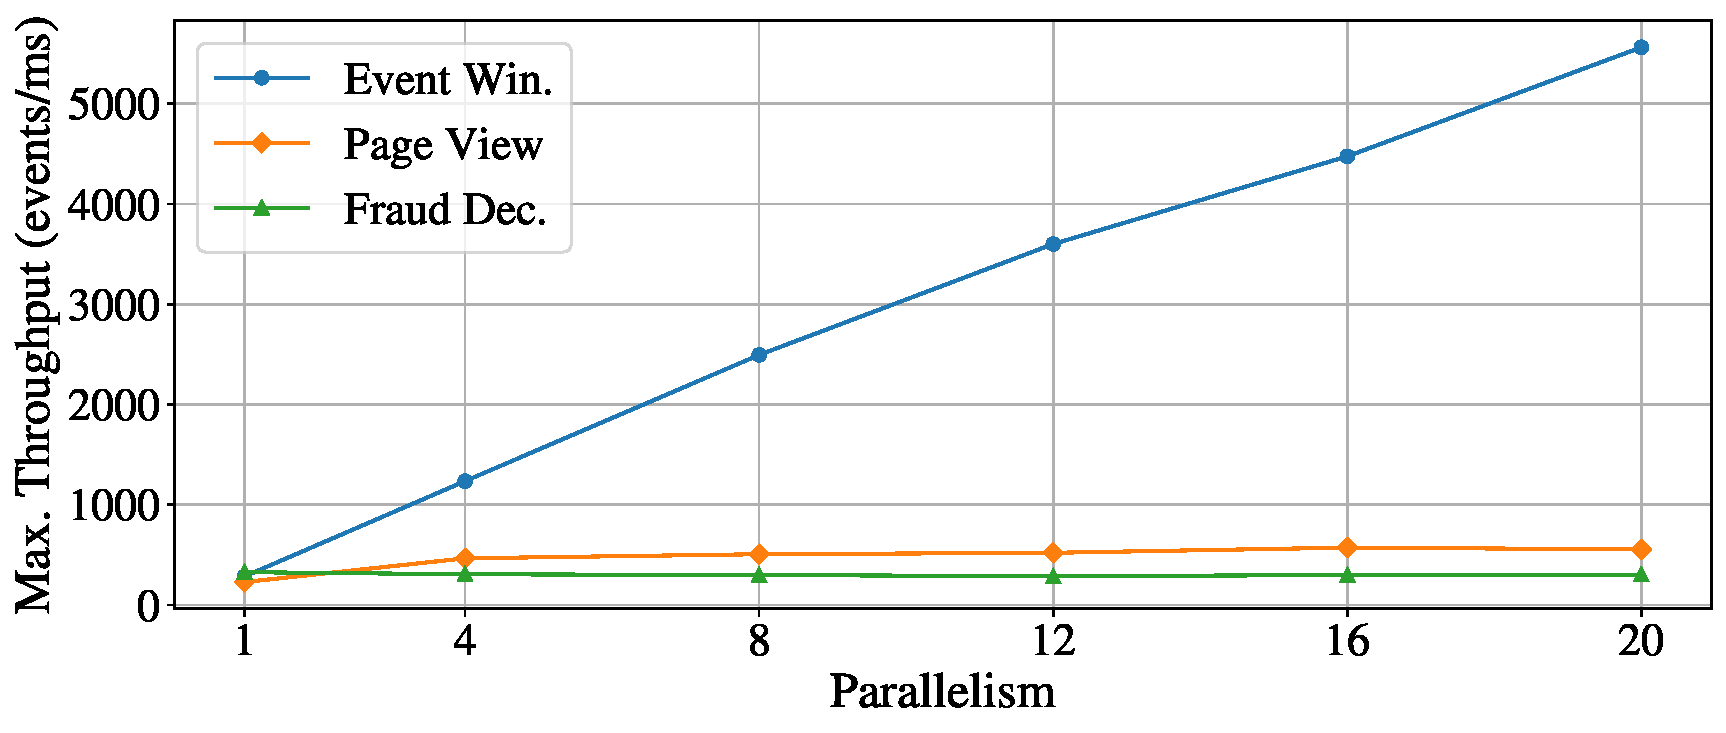
\includegraphics[width=0.48\columnwidth]{figures/dgs/flink_max_throughput_scaleup}
    ~
	  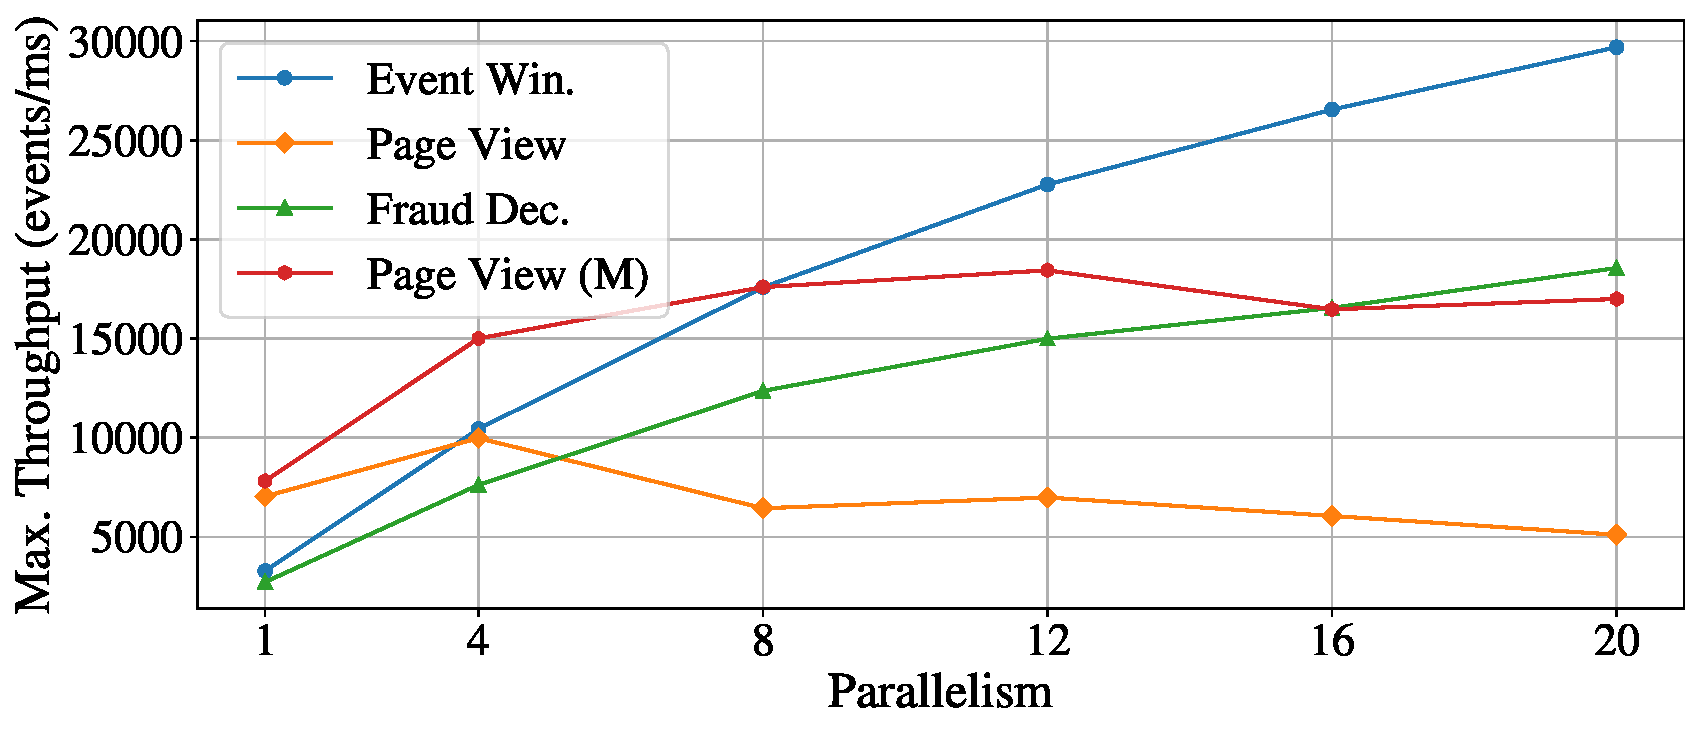
\includegraphics[width=0.48\columnwidth]{figures/dgs/timely_max_throughput_scaleup}
    \caption{
    Flink (left) and Timely (right) implementations maximum throughput increase with increasing parallel nodes for the three applications that require synchronization.
	% \caleb{Can we put these side by side? The figure is not very aesthetically pleasing right now.}
  % \kk{It is true that it is not pleasing, but putting them side by side will make the fonts too small.}
    % \kk{Include more summarization numbers in the prose.}
	% \str
	% \caleb{todo Konstantinos: can you remove the manual from Timely?}
    }
    \label{fig:existing-implementations-scaling}
\end{figure}


\begin{figure}[t]
  \centering
  \footnotesize{}
\begin{verbatim}
updates.broadcast().filter(move |x| {
    x.name == page_partition_function(NUM_PAGES, worker_index)
});
\end{verbatim}
\caption{Snippet of the manual (M) Timely implementation of the Page View example.
This violates \textbf{PIP2} since it explicitly references the physical partitioning of input streams
(\texttt{page\_partition\_function}) and the index of the worker that processes each stream (\texttt{worker\_index}).
}
\label{fig:timely-snippet}
\end{figure}


\begin{figure}[t]
    \centering
    \begin{subfigure}[b]{0.35\textwidth}
      \centering
      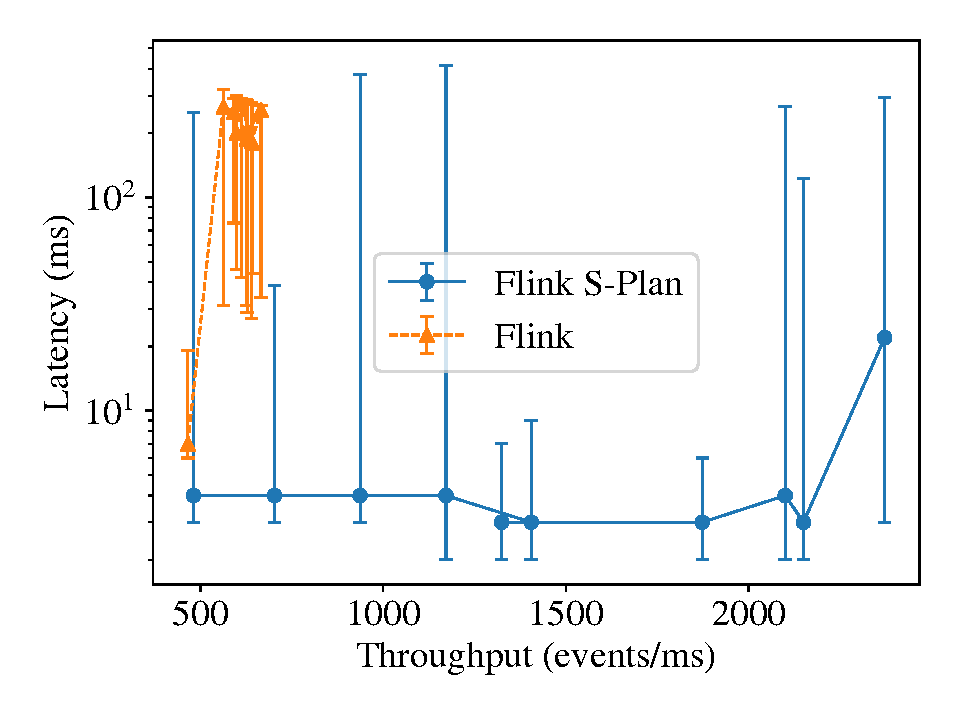
\includegraphics[width=\textwidth]{figures/dgs/pageview-flink-splan.pdf}
      \caption{Page-view Join.}
      \label{fig:synchronization-plan-page-view-join-throughput}
    \end{subfigure}
    \hspace{0.05\textwidth}
    \begin{subfigure}[b]{0.35\textwidth}
      \centering
      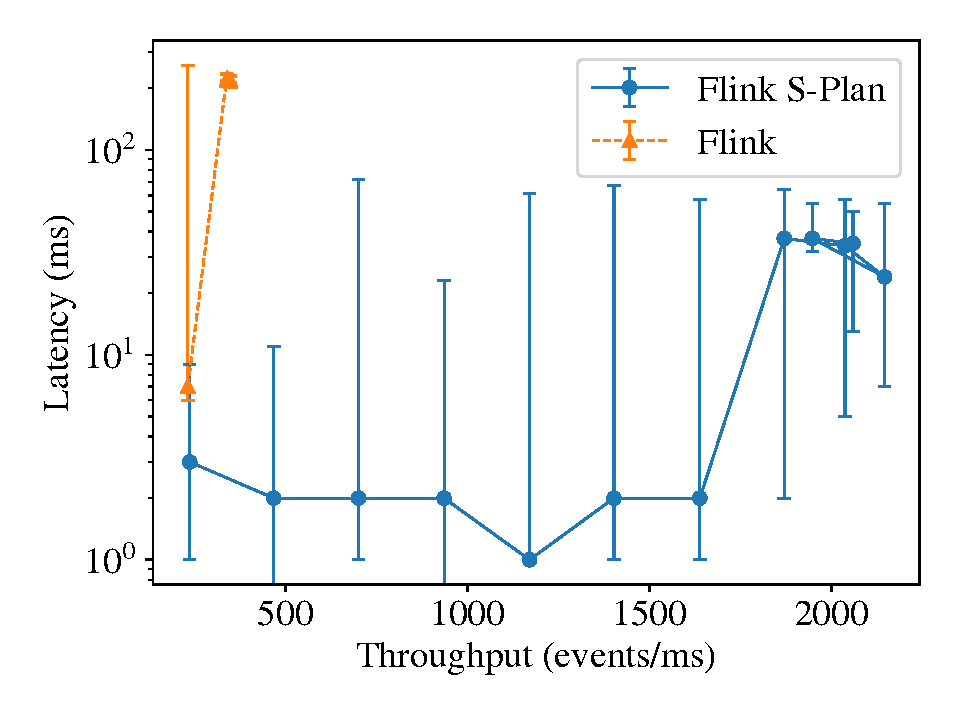
\includegraphics[width=\textwidth]{figures/dgs/frauds-flink-splan.pdf}
      \caption{Fraud Detection.
    %   Input rates from \todo{X} to \todo{Y}.
    %   \todo{12} nodes.
      }
      \label{fig:synchronization-plan-fraud-detection-throughput}
    \end{subfigure}
    \caption{
      Throughput (x-axis) and 10th, 50th, 90th percentile latencies on the y-axis for increasing input rates (from left to right) and 12 parallel nodes. Flink represents the parallel implementation produced automatically, and Flink S-Plan represents the synchronization plan implementation.
      }
    \label{fig:synchronization-plan-throughputs-flink}
\end{figure}

\begin{figure}
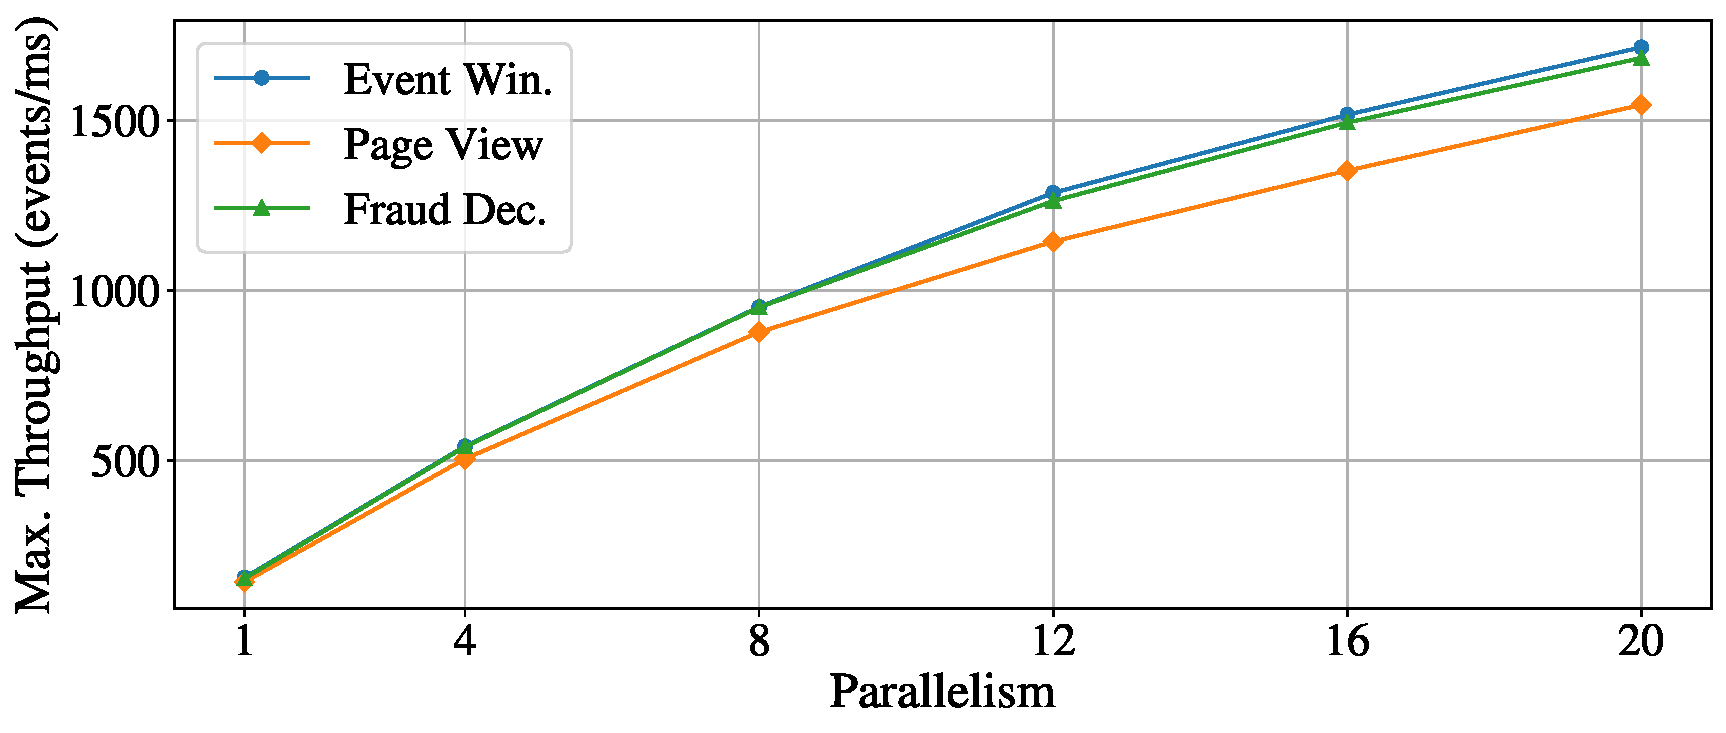
\includegraphics[width=\linewidth]{figures/dgs/flumina_max_throughput_scaleup.pdf}
\captionof{figure}{
DGSStream maximum throughput increase with increasing parallel nodes for the three applications that require synchronization.}
\label{fig:flumina-scaling}
\end{figure}
